\documentclass[../main.tex]{subfiles}
\begin{document}

\section[Однородное волновое уравнение в \texorpdfstring{$\R^3$}{R\textasciicircum 3}]{Формула Пуассона-Кирхгофа решения задачи Коши для однородного волнового уравнения в $\R^3$. Существование классического решения этой задачи.}
% Затехал: Погодин Роман
\begin{theorem}[Из курса мат. анализа]
Пусть 
$\Omega_x\subset\R^n,\ \Omega_y\subset\R^m$ -- ограниченные области,
$f(x,y)\colon \overline{\Omega}_x \times \overline{\Omega}_y \rightarrow \R,\ 
f \in C \brk*{ \overline{\Omega}_x\times\overline{\Omega}_y }$. 
Тогда 
$J(y) = \displaystyle\int\limits_{\Omega_x} f(x,y)\, dx\ 
\in C \brk*{ \overline{\Omega}_y }$. \\
%
Если к тому же 
$\dfrac{\partial f}{\partial y_k} 
\in C \brk*{ \overline{\Omega}_x\times\overline{\Omega}_y }$, 
то $J(y)$ имеет непрерывную на $\overline{\Omega}_y$ частную производную $\pd{J(y)}{y_k}$, 
которая равна $\displaystyle\int\limits_{\Omega_x} \pd{f}{y_k} (x,y)\, dx.$
\end{theorem}

\begin{lemma}
Пусть $g(\tau, \xi) \in C^{0,\, p}_{\tau,\, \xi} \,\brk[c]!{\tau \geq 0,\ \xi \in \R^3}$. Введём $u_g(t, x, \tau)\colon$
\[
u_g(t,x,\tau) \coloneqq \frac{1}{4\pi a^2t}\oiint\limits_{|\xi - x|=at}g(\tau, \xi)\, dS_{\xi}\, , \qquad a>0,\ t> 0,\ x\in \R^3,\ \tau \geq 0,\ \xi\in\R^3
\]
Тогда
\begin{enumerate}

\item $u_g \in C^{p,\, p,\, 0}_{t,\, x,\, \tau}\, \brk[c]!{\mathbf{t \geq 0},\ x \in \R^3, \tau \geq 0}$

\item $\lim\limits_{t\rightarrow +0} u_g(t,x,\tau) = 0$

\item При $p\geq 1$ $\lim\limits_{t\rightarrow +0}\dfrac{\partial u_g}{\partial t}=g(\tau, x)$

\end{enumerate}
\end{lemma}

(Под $C^{p,\, p,\, 0}_{t,\, x,\, \tau}$ подразумевается, что $D_{t,x}^{\alpha}\, u_g(t,x,\tau) \in C \Forall\alpha\colon |\alpha| \leq p$)
\footnote{Если расписать мультииндексы: \ $\partial^{\alpha_0}_t    \, 
\partial^{\alpha_1}_{x_1} \, 
\partial^{\alpha_2}_{x_2} \,
\partial^{\alpha_3}_{x_3} \; 
u_g(t, x, \tau) 
\in C \;\Forall \alpha_i \colon \sum\limits_{i=0}^{3} \alpha_i \leq p$}

\begin{proof} Докажем отдельно все три утверждения.
%
\begin{enumerate}
\item Сведем интеграл к интегралу по единичной сфере с центром в нуле с помощью такой замены:
\[
\eta = \frac{\xi - x}{at}
\ \Rightarrow\ 
\xi = x+at\eta,\ |\vec{\eta}|=1.
\]
В таком случае элемент площади $dS_{\xi}=(at)^2dS_{\eta}$. Во введенном выше интеграле получим 
\[
u_g(t,x,\tau) = \frac{(at)^2}{4\pi a^2t}
\oiint\limits_{|\eta|=1}   g(\tau,\, x+at\eta)\,   dS_{\eta} 
= t J_g(t,x,\tau),
\]
где $\displaystyle J_g(t,x,\tau) = \frac{1}{4\pi}
\oiint\limits_{|\eta|=1}   g(\tau,\, x+at\eta)\,   dS_{\eta}$

Теперь интеграл уже по фиксированному множеству. Все выкладки справедливы при $t>0$. Функция
\[
\tilde{g}(t,x,\eta,\tau) = g(\tau,\, x+at\eta)\ 
\in C\, \{t \geq 0,\   x\in\R^3,\   |\eta| = 1,\   \tau \geq 0\}.
\]
Тогда по теореме из начала билета 
$J_g(t,x,\tau) \in C\, \{t\geq 0,\   x\in\R^3,\   \tau \geq 0\}.$

Аналогично будет для производных в силу второй части той же теоремы и наличия соответствующих производных у функции $g$.

\item $\lim\limits_{t\rightarrow +0} U_g(t,x,\tau)
     = \lim\limits_{t\rightarrow +0} t J_g(t,x,\tau)
     = \lim\limits_{t\rightarrow +0} t 
 \cdot \lim\limits_{t\rightarrow +0} J_g(t,x,\tau) = 0$ 
 (последний предел конечен в силу непрерывности).

Можно записать
\[
U_g(t,x,\tau) 
= \begin{cases}
    u_g(t,x, \tau), &t>0,\\
    0, &t=0,
  \end{cases} \quad 
\in C \brk*{ \overline{\Omega} },
\]
где последнее включение означает непрерывные в области и непрерывно продолжимые на границу функции.

\item При $p\geq 1$ запишем следующее:
\begin{equation*}
\begin{split}
&\lim\limits_{t\rightarrow +0} \pd{}{t} u_g(t,x, \tau) 
=\lim\limits_{t\rightarrow +0} \pd{}{t} \brk[s]*{t J_g(t,x,\tau)}
=\lim\limits_{t\rightarrow +0} J_g(t,x,\tau)
+\cancelto{0}
{\lim\limits_{t\rightarrow +0} t \cdot \pd{}{t} J_g(t,x,\tau)} = \\
%
&= J_g(0, x, \tau) = \frac{1}{4\pi}
\oiint\limits_{|\eta|=1}   g(\tau, x+at\eta)\,   dS_{\eta }
\Biggr|_{t=0}
= g(\tau, x) \frac{1}{4\pi}
\oiint\limits_{|\eta|=1}   dS_{\eta}   =   g(\tau, x).
\end{split}
\end{equation*}
\end{enumerate}
\end{proof}

\imaginarySubsection{Формула Пуассона-Кирхгофа}

Перейдем к решению задачи Коши
\begin{equation}
\begin{cases}
  u_{tt} - a^2\Delta u = 0,   \quad t>0,\   x \in \R^3, \\
  \eval{ u }_{t=0} = 0,   \\
  \eval{u_t}_{t=0} = u_1(x).
\end{cases}
\label{eq::7::cauchy}
\end{equation}

\begin{theorem}[Формула Пуассона-Кирхгофа]
Пусть $u_1(x) \in C^2(\R^3)$. Тогда 
\[
u(t,x) = \frac{1}{4\pi a^2t}
\oiint\limits_{|\xi-x|=at}  u_1(\xi)\,  dS_{\xi}   \quad
\in\: C^2\,   \{t\geq 0,\   x \in \R^3 \}
\]
является классическим решением задачи \eqref{eq::7::cauchy}.
\end{theorem}

\begin{proof}
В силу леммы имеем 
$\eval{u}_{t=0} = 0;\ \eval{u_t}_{t=0} = u_1$.

Т.к. $u_1 \in C^2(\R^3),\ u \in C^2\,\{t\geq 0, x\in\R^3\}$, то сделаем замену переменной:
\[
u(t,x) = \frac{t}{4\pi}
\oiint\limits_{|\eta|=1}  u_1(x+at\eta)\,  dS_{\eta}.
\]
Осталось только проверить, что $u$ удовлетворяет уравнению
\[
\Delta_x u(x,t) 
= \frac{t}{4\pi}
  \oiint\limits_{|\eta|=1}   \Delta_{\xi} u_1(x+at\eta)\,  dS_{\eta}
= \frac{1}{4\pi a^2t}
  \oiint\limits_{|\xi-x|=at}  \Delta_{\xi} u_1(\xi)\,  dS_{\xi}.
\]
При $t>0$ (использовано $\vec{n} 
     = \dfrac{\xi-x}{|\xi-x|} 
     = \dfrac{\xi-x}{at}   =  \eta$):
\begin{equation*}
\begin{split}
%
&u_t(x,t) = \frac{1}{4\pi}
\oiint\limits_{|\eta|=1}  u_1(x+at\eta)\,  dS_{\eta}
+\frac{ta}{4\pi}
\oiint\limits_{|\eta|=1}
      \sum\limits_{k=1}^3 
      \pd{u_1}{\xi_k} (x+at\eta) \eta_k 
      \cdot dS_{\eta} 
 = \\[0.75em]
%
&=\frac{u(x,t)}{t} + \frac{ta}{4\pi}
\oiint\limits_{|\eta|=1}
       \sum\limits_{k=1}^3 
       \pd{u_1}{\xi_k} (\xi)  n_k(\xi)
       \cdot dS_{\eta}
%
=\frac{u(x,t)}{t} + \frac{1}{4\pi at}
\oiint\limits_{|\xi-x|=at}
       \pd{u_1}{\vec{n}}(\xi) 
       \cdot dS_{\xi}
%
=\frac{u(x,t)}{t} + \frac{1}{4\pi at} I
%
\end{split}
\end{equation*}
Заметим, что
\[
 \iiint\limits_{|\xi-x|<at}  \Delta_{\xi}  u_1(\xi)\,   d\xi 
=\iiint\limits_{|\xi-x|<at}    \div  (\nabla u_1)\,     d\xi 
=\oiint\limits_{|\xi-x|=at}  (\nabla u_1,\, \vec{n})\,  dS_{\xi }
=\oiint\limits_{|\xi-x|=at}     \pd{u_1}{\vec{n}}\,     dS_{\xi }=I
\]
Тогда получим 
$$
u_t = \frac{u}{t} + \frac{1}{4\pi at}
 \iiint\limits_{|\xi-x|<at}  \Delta_{\xi}  u_1(\xi)\,   d\xi \\
%
=\frac{u}{t} + \frac{1}{4\pi at}
\int\limits_0^{at} 
  \left[
    \oiint\limits_{|\xi-x|=\rho}  \Delta_{\xi} u_1(\xi)\,  dS_{\xi}
  \right] d\rho \\
%
=\frac{u}{t} + \frac{1}{4\pi at}
\int\limits_0^{at}  \phi(\rho)\,  d\rho
$$

\begin{equation*}
\begin{split}
&u_{tt}(x,t) = \pd{}{t}
  \left[
    \frac{u}{t} + \frac{I}{4\pi at} 
  \right]
= \frac{u_t}{t} - \frac{u}{t^2}
  - \frac{I}{4\pi at^2} + \frac{I_t}{4\pi at} 
= \frac{1}{t} \cdot \left( \frac{u}{t} + \frac{I}{4\pi at} \right)
  - \frac{u}{t^2} - \frac{I}{4\pi at^2} 
  + \frac{I_t}{4\pi at} = \\
%
&=\frac{I_t}{4\pi at} 
= \frac{1}{4\pi at} \pd{}{t}
  \int\limits_0^{at}  \phi(\rho)\,  d\rho 
= \frac{1}{4\pi at} a \phi(at)
= \frac{1}{4\pi t}
  \oiint\limits_{|\xi-x|=at}  \Delta_{\xi}  u_1(\xi)\,  dS_{\xi}.
\end{split}
\end{equation*}
%
Итак, $u(x, t)$ -- классическое решение.
\end{proof}

Рассмотрим
\begin{equation}
\begin{cases}
  u_{tt}-a^2\Delta u=0,\quad t>0,\, x\in \R^3\\
  \eval{u}_{t=0}=u_0(x) \in C^3(\R^3),\\
  \eval{u_t}_{t=0}=0.
\end{cases}
\label{eq::7::cauchy2}
\end{equation}

Введем $v(t,x)$:
\[
\begin{cases}
  v_{tt} - a^2 \Delta v=0,  \quad t>0,\ x\in \R^3 \\
  \eval{ v }_{t=0} = 0, \\ 
  \eval{v_t}_{t=0} = u_0(x).
\end{cases}
\]

Эту задачу мы уже решили. Так как $u_0\in C^3(\R^3)$, 
имеем $v\in C^3\, \{t\geq 0,\  x\in\R^3\}$.

\begin{statement}
$u(x,t) \equiv v_t(x, t) \in C^2\, \{t\geq 0,\  x\in\R^3 \}$ 
дает решение задачи \eqref{eq::7::cauchy2}.
\end{statement}

\begin{proof}$\ $
\begin{enumerate}

\item  $u_{tt} - a^2 \Delta u 
= \partial_t (v_{tt} - a^2 \Delta v) 
= \partial_t\: 0 
= 0$

\item $ \eval{u}_{t=0} = \eval{v_t}_{t=0} = u_0(x) $

\item $\eval{u_t}_{t=0} = \eval{v_{tt}}_{t=0} = a^2 \Delta \eval{v}_{t=0} = 0$ 
%
(на гиперплоскости  $t=0  \colon\ 
                 \eval{v}_{t=0} \equiv 0\ \Rightarrow\ 
 \eval*{\pd{v}{x_i}}_{t=0} \equiv 0\ \Rightarrow\ 
\eval*{\pd[2]{v}{x_i}}_{t=0} \equiv 0. $ 
\; При этом $v_t$ может быть ненулевой.)

\end{enumerate}
\end{proof}

Мы доказали следующую теорему:
\begin{theorem}
Функция $u(t,x) = \pd{}{t}
  \left[
    \dfrac{1}{4\pi a^2t}\displaystyle\oiint\limits_{|\xi-x|=at}  u_0(\xi)\,  dS_{\xi } 
  \right],\ 
t \geq 0,\   x\in\R^3$,  где $u_0 \in C^3(\R^3)$, \\[1em]
является классическим решением задачи \eqref{eq::7::cauchy2}. 
\end{theorem}


\Subsection{Принцип Гюйгенса}

\begin{statement}[Принцип Гюйгенса]
    Возмущение, локализованное в пространстве (трёхмерном), приводит к действию, локализованному во времени.
\end{statement}

% Требуется отсутствие источников: $f \equiv 0$ -- и ограниченность носителей функций $u_0$ и $u_1$:
Требуется, чтобы 
источники отсутствовали, т.е.
$f \equiv 0$, а носители функций $u_0$ и $u_1$ были ограничены, откуда
$$\supp u_0 \ \cup\ \supp u_1 = M \text{ -- компакт}$$

Фиксируется произвольная точка $x_0 \in \R^3$.

По формуле Кирхгофа функция $u(t, x_0)$ может быть ненулевой только внутри отрезка времени
$$
\text{от \ } t_\text{start} = \frac{1}{a} \cdot \inf_{y\in M}|y-x_0|
\qquad \text{ \ до \ } t_\text{end} = \frac{1}{a} \cdot \sup_{y \in M}|y-x_0|
$$
(иначе под интегралами тождественный нуль).

У такого конечного возмущения есть передний и задний фронт:
\vspace{0.7em}

\centering
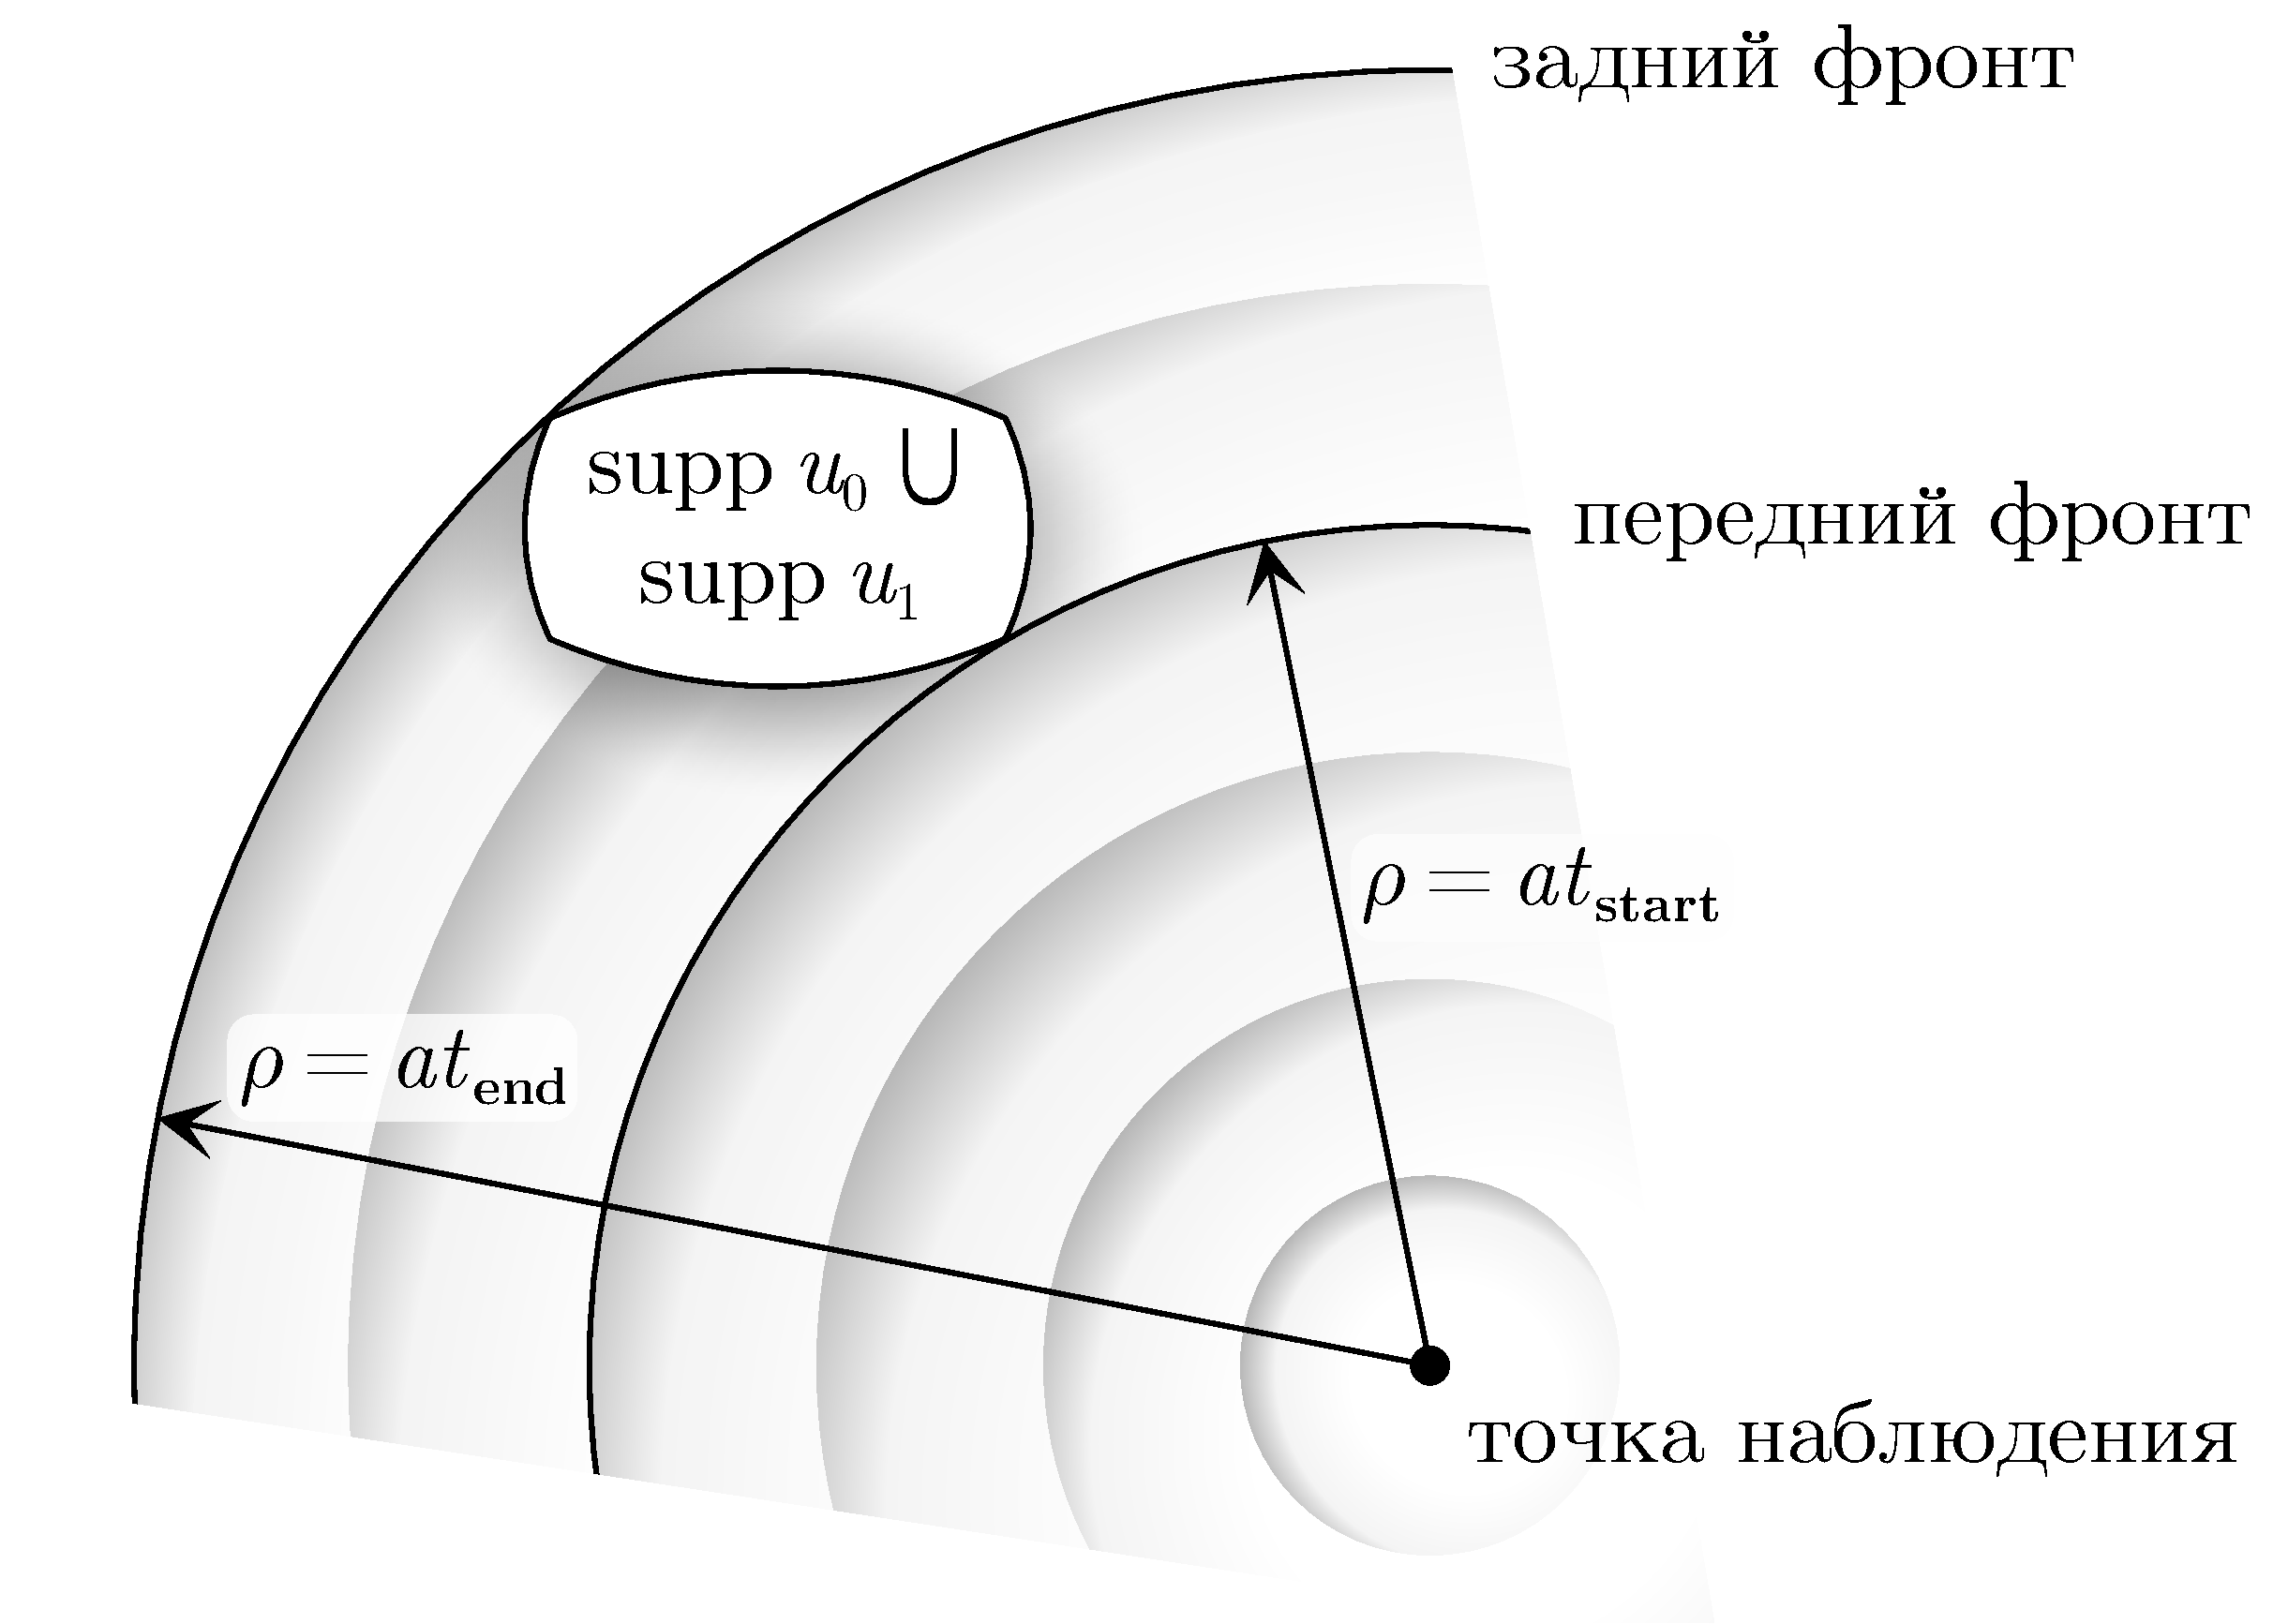
\includegraphics[width=0.45\textwidth]{./pic 7.pdf}

Значение $u(t,x_0)$ \ $\sim$ \ интеграл по сфере радиусом $|x_0 -\xi| = \rho = at$

\end{document}